\documentclass[..\report.tex]{subfiles}

\begin{document}

\section{Barotropic Vorticity Diagnostics}
\label{SEC:Diagnostics}

Our aim is to understand the reasons behind the improved representation of the Gulf Stream in higher-resolution models. The first steps towards this will be trying to identify the key processes which are not being resolved in the coarser models. To investigate this, we use barotropic vorticity diagnostics to identify the leading terms of the momentum equation.

These barotropic vorticity diagnostics have been used by \citet{Bell1999}, \citet{Gula2014} and \citet{Yeager2015}, among others, to investigate the driving forces behind the vorticity budgets in the North Atlantic.
Using the \gls{NEMO} model, we will implement these diagnostics across models of different resolutions to allow for a comparison. This will help to identify the cause of the contrasting representations of the Gulf Stream in different resolution models. \par

Two different diagnostics will be calculated on each of the seven contributing terms to the momentum equations shown in equation (\ref{EQN:NEMOPrognostic}). The methods are similar to the approach taken in section \ref{SSEC:EffectsOfTopography} to find the JEBAR and bottom pressure torque terms and involve taking the curl of the vertically averaged and vertically integrated contributions.\par

Examining and comparing the results will help to highlight the leading terms driving the flow in different regions of the Gulf Stream. This may highlight key areas of bathymetry or emphasise the importance of the interaction with the \gls{DWBC}.

\subsection{\gls{NEMO} Ocean Model}
\label{SSEC:NEMO}

As the barotropic vorticity diagnostics are being implemented in the \gls{NEMO} model, it seems sensible to first introduce the model in a little more detail. \par
\gls{NEMO} is a framework designed to allow for a flexible study of the ocean, it's dynamics and it's interaction with other climate systems \citep{Madec2011}. \par

The framework of \gls{NEMO} allows the model to be configured in a variety of ways, choosing the resolution, numerical schemes and vertical coordinates according to requirements. As discussed in section \ref{SEC:ModellingGulfStream}, the representation of the Gulf Stream can vary greatly depending on various aspects of the model chosen. \citet{Scaife2011a} showed that the resolution can play a big role in the simulated path of the Gulf Stream. Whereas, \citet{Ezer2016b} showed that the Gulf Stream is sensitive also to the choice of vertical coordinates and bathymetrical representation. It is suitable then, for our requirements, as it will allow comparisons between a variety of different configurations in a way which can be problematic for most modellers (as noted by \citet{Ezer2016b}).\par

Within \gls{NEMO}, there are many different engines designed to model different aspects of the ocean, these are \myacr{OPA}, which models the ocean dynamics and thermodynamics; \myacr{LIM}, which models the sea-ice dynamics and thermodynamics; and \myacr{TOP}, modelling the biogeochemistry. For our purposes we are interested in \gls{OPA}, which will we will run off the MONSooN super computer.\par
We can further narrow our interests for the current investigation within \gls{OPA} down to the routines focusing on the ocean dynamics. This part of the model is located within the \myacr{DYN} directory of the code and is responsible for the momentum equations, which are key to the barotropic vorticity diagnostics and are the focus of this section. \par

The prognostic ocean dynamics equations used by \gls{NEMO} (where $(NXT)$ stands for the next time step) are 
\begin{equation}
\begin{split}
    NXT = \underbrace{(VOR+KEG+ZAD)}_\text{Coriolis \& advection} + \underbrace{HPG+SPG}_\text{pressure gradient contributions} \\
    +\underbrace{LDF}_\text{lateral diffusion} +\underbrace{ZDF}_\text{vertical diffusion}.
\end{split}
\label{EQN:NEMOPrognostic}
\end{equation}


Here the Coriolis and advection terms are split into three parts: the vorticity $(VOR)$, the kinetic energy $(KEG)$ and the vertical advection $(ZAD)$.
In place of the Coriolis and advection terms shown here, in the flux formation, they can be replaced by a Coriolis and advection term $(COR + ADV)$, however, for our purposes we will be using the terms shown in equation (\ref{EQN:NEMOPrognostic}). The pressure gradient contributions consist of the hydrostatic pressure gradient $(HPG)$ and the surface pressure gradient $(SPG)$, and we also have the lateral $(LDF)$ and vertical diffusion $(ZDF)$ terms \citep{Madec2011}.
%\todo{Put citation elsewhere?}

Currently the diagnostics are being added to a $0.25\degree$ model using the z-coordinate bathymetry with partial steps (shown in Figure \ref{FIG:Coords} (b)).
Following the successful implementation of these diagnostics in one model formulation in \gls{NEMO}, the intention is to then compare the results gained from running the calculations across different model resolutions and possibly different choices of vertical coordinates.

This could build on the review by \citet{Ezer2016b} by allowing for a more controlled comparison between models and allow an easier comparison and analysis of the results. Figure \ref{FIG:Ezer2016bFig8} \citep[Fig. 8]{Ezer2016b} shows the effect that the choice of model grid can have on the balance of the barotropic vorticity budget. With the various available configurations of \gls{NEMO}, it will be interesting to further investigate this within a more controlled set up.

\begin{figure}[t]
    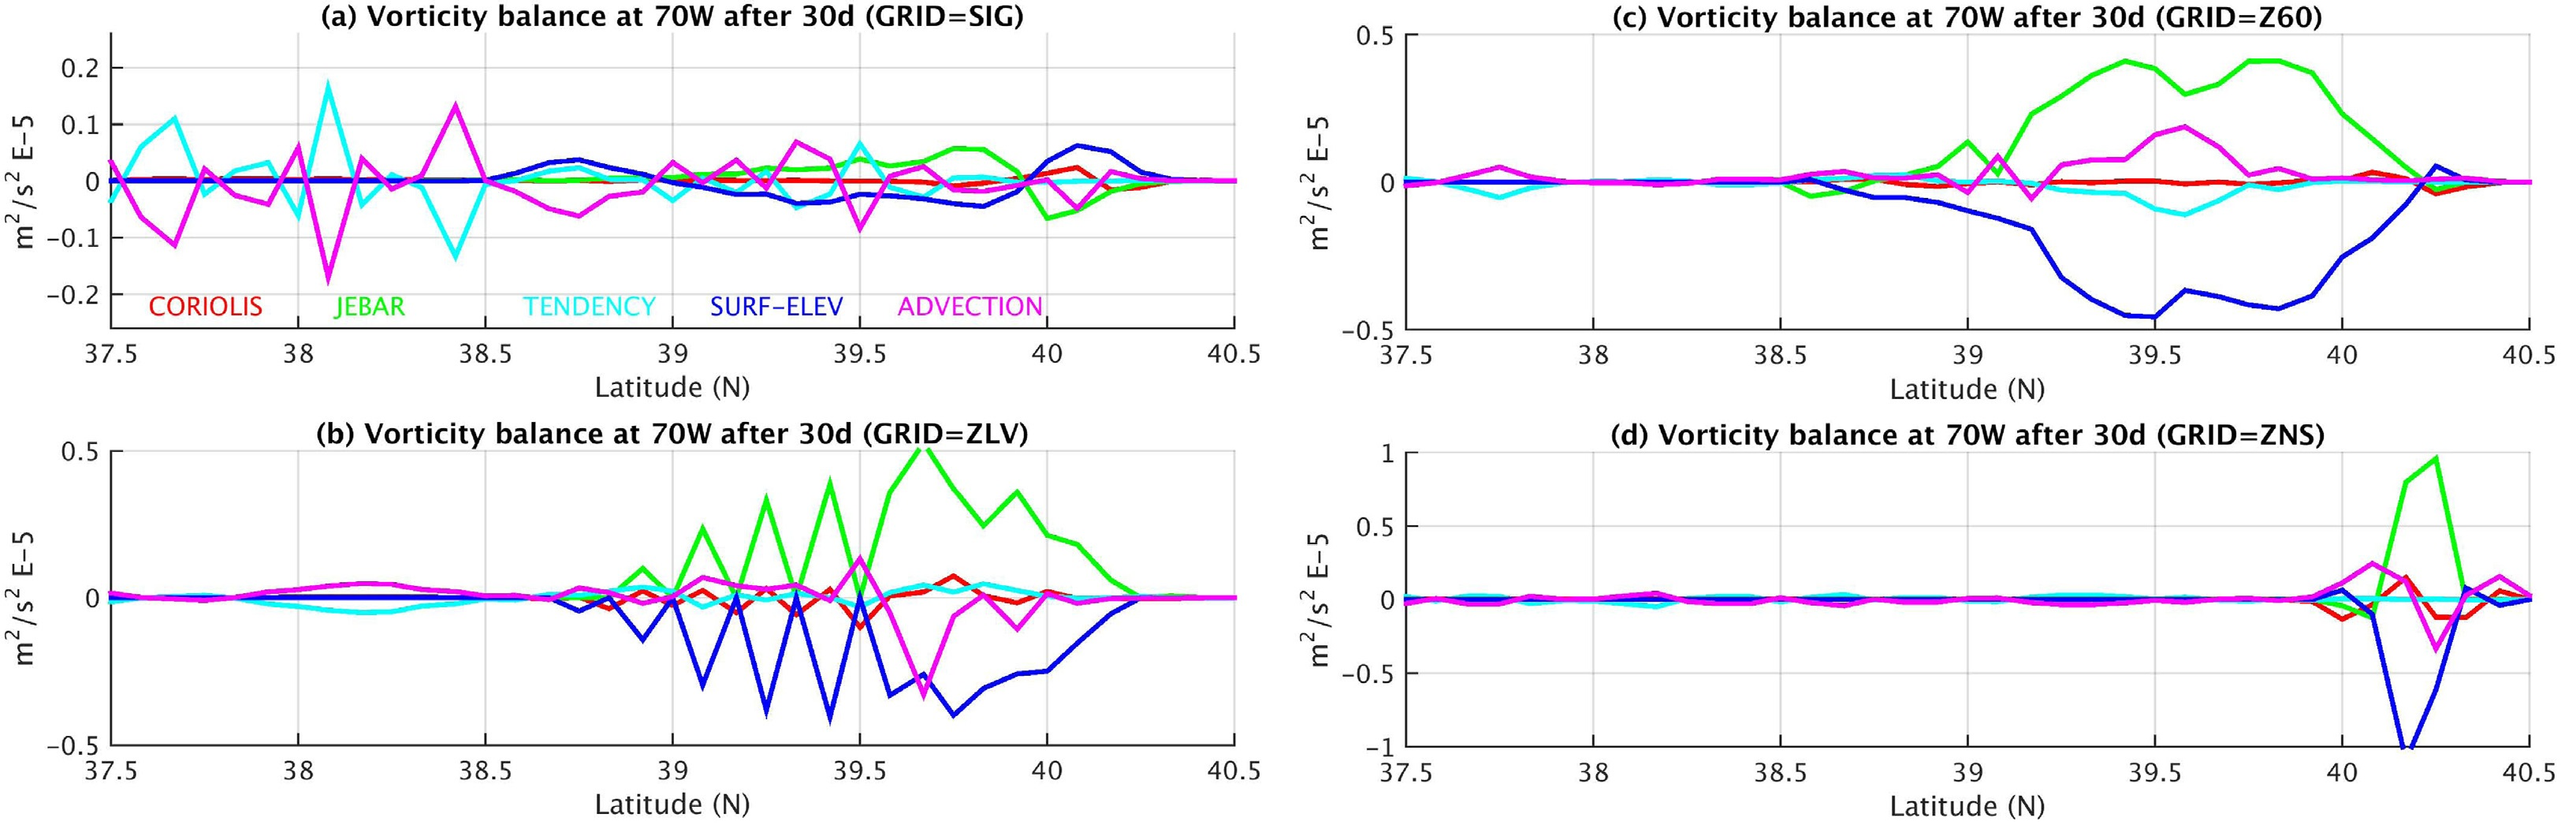
\includegraphics[width=\linewidth]{Figures/Ezer2016bFig8.jpg}
    \caption{This is an example of the kind of results available from barotropic vorticity diagnostics \citep[Fig 8.]{Ezer2016b}. Leading terms of the vorticity balance equation at 70$\degree$W after 30 days for experiments: (a) SIG (sigma coordinates), (b) ZLV (z-level coordinates with 21 layers), (c) Z60 (z-level coordinates with 61 layers) and (d) ZNS (z-level coordinates with no continental slope). Note the different scale in each panel. Each term has different color as indicated in (a).}
    \label{FIG:Ezer2016bFig8}
\end{figure}


\subsection{Barotropic Vorticity Diagnostics}
\label{SSEC:BVDiagnostics}


New code has been added to the \gls{NEMO} model to calculate the two barotropic vorticity diagnostics. The two different diagnostics come from the derivations of the \gls{JEBAR} and bottom pressure torque terms discussed in section \ref{SSEC:EffectsOfTopography}. As each contribution to the momentum trend is calculated, it is passed to the subroutine which then calculates the required values.

The subroutine first calculates the vertical integral of the contribution, $\bar{u}$ and $\bar{v}$, over the height of the water column from the depth, $-H$, to the sea surface level $\eta$,
\begin{equation}
    \bar{u} = \int_{-h}^{\eta} u \,\text{d}z \,,\quad \bar{v} = \int_{-h}^{\eta} v \,\text{d}z 
    \label{UVBar}
\end {equation}


and then divides through by the height of the water column to obtain the vertical averages $\langle\bar{u}\rangle$ and $\langle\bar{v}\rangle$,
\begin{equation}
	\langle\bar{u}\rangle = \frac{1}{\eta + h}\int_{-h}^{\eta}u \,\text{d}z \,,\qquad \langle\bar{v}\rangle = \frac{1}{\eta + h}\int_{-h}^{\eta}v \,\text{d}z.
\label{UVBar}
\end{equation}


The curl of each of these values is then calculated to attain the two desired diagnostics
\begin{equation}
    \Omega = \frac{\partial \bar{v}}{\partial x} - \frac{\partial \bar{u}}{\partial y}
    \label{EQN:IntegratedDiagnostic}
\end{equation}


\begin{equation}
    \Omega_{avg} = \frac{\partial \langle\bar{v}\rangle}{\partial x} - \frac{\partial \langle\bar{u}\rangle}{\partial y}.
    \label{EQN:AveragedDiagnostic}
\end{equation}

    
Once the diagnostics have been calculated we can then compare the different contributions as done by \citet{Yeager2015} and \citet{Gula2014}. Using equation (\ref{EQN:Streamfunction}) we can also calculate the barotropic streamfunction driving the flow to gain further insight into the topological effects on the flow.


\end{document}
